% Digital Logic Report Template
% Created: 2020-01-10, John Miller

%==========================================================
%=========== Document Setup  ==============================

% Formatting defined by class file
\documentclass[11pt]{article}

% ---- Document formatting ----
\usepackage[margin=1in]{geometry}	% Narrower margins
\usepackage{booktabs}				% Nice formatting of tables
\usepackage{graphicx}				% Ability to include graphics

%\setlength\parindent{0pt}	% Do not indent first line of paragraphs 
\usepackage[parfill]{parskip}		% Line space b/w paragraphs
%	parfill option prevents last line of pgrph from being fully justified

% Parskip package adds too much space around titles, fix with this
\RequirePackage{titlesec}
\titlespacing\section{0pt}{8pt plus 4pt minus 2pt}{3pt plus 2pt minus 2pt}
\titlespacing\subsection{0pt}{4pt plus 4pt minus 2pt}{-2pt plus 2pt minus 2pt}
\titlespacing\subsubsection{0pt}{2pt plus 4pt minus 2pt}{-6pt plus 2pt minus 2pt}

% ---- Hyperlinks ----
\usepackage[colorlinks=true,urlcolor=blue]{hyperref}	% For URL's. Automatically links internal references.

% ---- Code listings ----
\usepackage{listings} 					% Nice code layout and inclusion
\usepackage[usenames,dvipsnames]{xcolor}	% Colors (needs to be defined before using colors)

% Define custom colors for listings
\definecolor{listinggray}{gray}{0.98}		% Listings background color
\definecolor{rulegray}{gray}{0.7}			% Listings rule/frame color

% Style for Verilog
\lstdefinestyle{Verilog}{
	language=Verilog,					% Verilog
	backgroundcolor=\color{listinggray},	% light gray background
	rulecolor=\color{blue}, 			% blue frame lines
	frame=tb,							% lines above & below
	linewidth=\columnwidth, 			% set line width
	basicstyle=\small\ttfamily,	% basic font style that is used for the code	
	breaklines=true, 					% allow breaking across columns/pages
	tabsize=3,							% set tab size
	commentstyle=\color{gray},	% comments in italic 
	stringstyle=\upshape,				% strings are printed in normal font
	showspaces=false,					% don't underscore spaces
}

% How to use: \Verilog[listing_options]{file}
\newcommand{\Verilog}[2][]{%
	\lstinputlisting[style=Verilog,#1]{#2}
}




%======================================================
%=========== Body  ====================================
\begin{document}

\title{ELC 2137 Lab 2: Transistor Logic Gates}
\author{Trevor Jackson, Carlos Hernandez, and Makenna Meyers}

\maketitle


\section*{Summary}

This lab introduced the idea of logic gates and transistors, which act like switches. Basic circuits, including a two pushbutton AND gate circuit, an inverter circuit, and a NOR gate circuit, were constructed to become familiar with gates and how they work. To further aid comprehension, current paths were drawn on instructor-given circuits. Said circuits are found in Figure \ref{fig:Circuit_Demonstration(1)} and  Figure \ref{fig:Circuit_Demonstration(2)}. After mastering these basic skills, a final gate was constructed by combining two inverters and the previously made NOR gate. This combination of gates produced an AND gate, and the truth table describing it can be found in Table \ref{tbl:truth_table}.

\section*{Q\&A}

\begin{enumerate}
	\item What logic operation does the final gate implement?
	
	The final gate applies the AND operation.

\end{enumerate}

\section*{Results}

In Table \ref{tbl:truth_table}, A and B refer to switches in the Final Gate circuit found in Figure \ref{fig:Circuit_Demonstration(2)}. C refers to the LED light in this circuit.

\begin{table}[ht]\centering
	\caption{Truth Table for the Final Gate}
	\label{tbl:truth_table}
	\begin{tabular}{cc|c}
    	\toprule
    	A & B & C \\
    	\midrule
    	0 & 0 & 0 \\
    	0 & 1 & 0 \\
    	1 & 0 & 0 \\
    	1 & 1 & 1 \\
    	\bottomrule
    \end{tabular} 
\end{table}

\begin{figure}\centering
	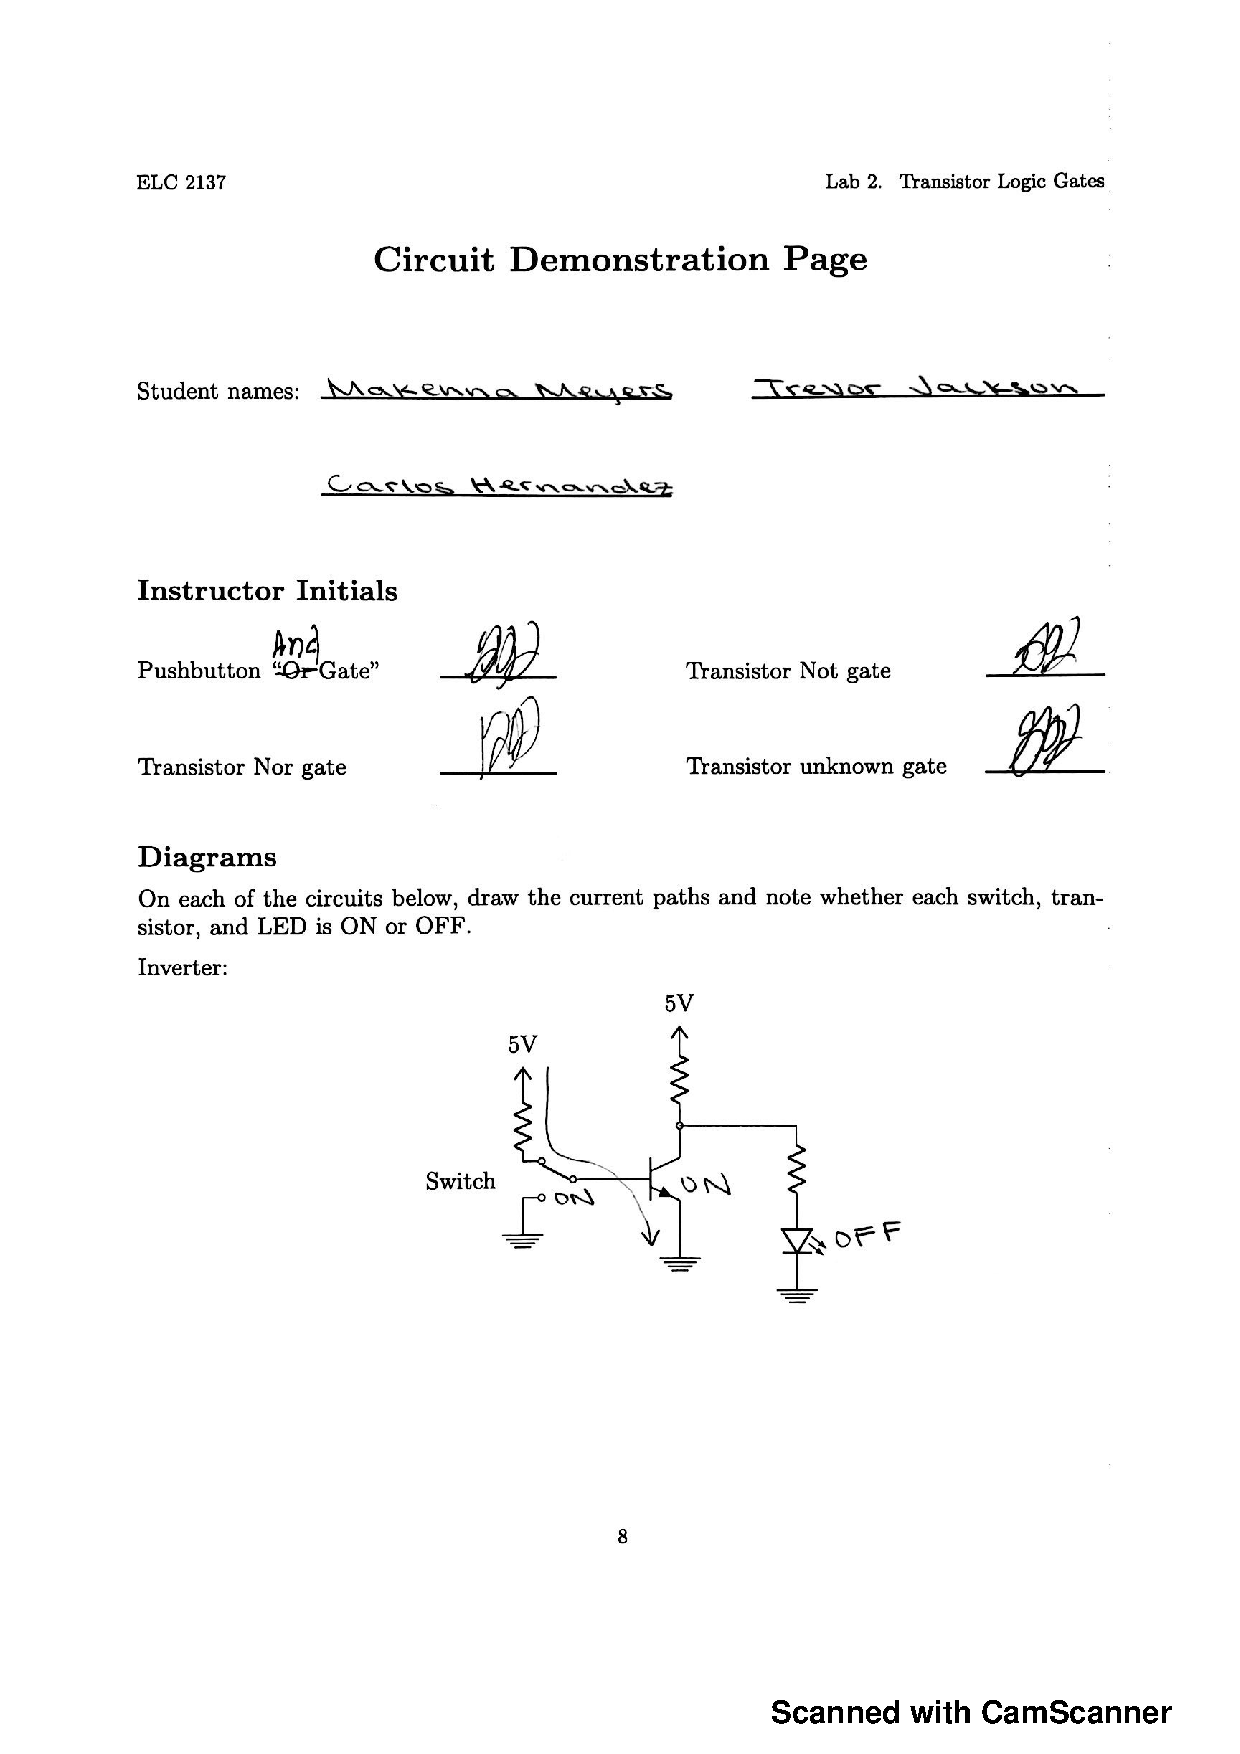
\includegraphics[width=0.8\textwidth,trim=2cm 6cm 2cm 2cm,clip]{Circuit_Demonstration} 
	\caption{In-Class Circuit Demonstration Page 1}
	\label{fig:Circuit_Demonstration(1)}
\end{figure}	

When the switch in the Inverter circuit in Figure \ref{fig:Circuit_Demonstration(1)} is on, current flows to ground and not through the LED light, so the light remains off. If the switch were to be turned off, current would flow through the light, turning it on.
	
	\clearpage
	
\begin{figure}\centering
	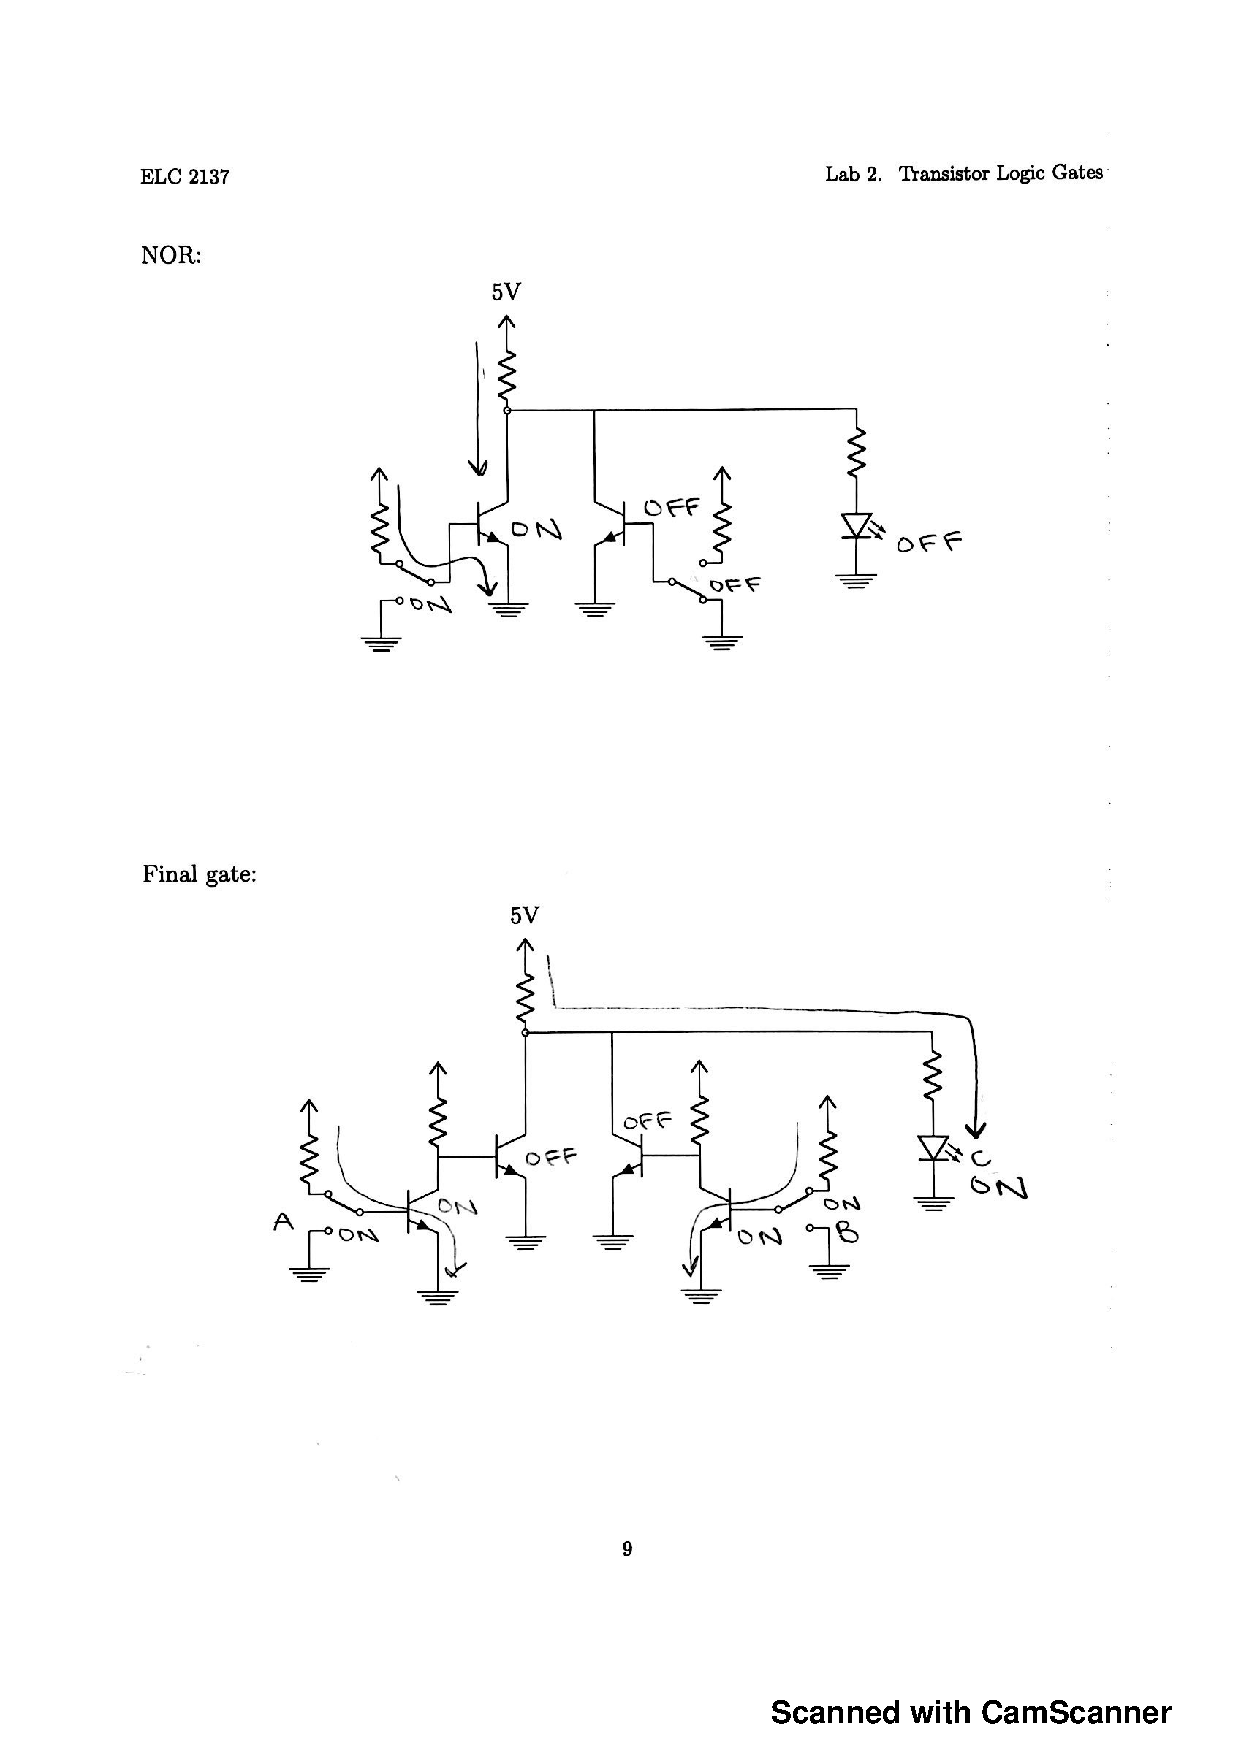
\includegraphics[width=0.8\textwidth,trim=2cm 6cm 2cm 2cm,clip]{Circuit_Demonstration(2!)}
	\caption{In-Class Circuit Demonstration Page 2}
	\label{fig:Circuit_Demonstration(2)}	
\end{figure}

\clearpage

When one switch in the NOR gate circuit in Figure \ref{fig:Circuit_Demonstration(2)} is on, current flows to ground and not through the LED light, so the light remains off. If the switch were to be turned off, current would flow through the light, turning it on. Turning both switches on would also prevent current from flowing through the light, keeping the light turned off. Only if both switches were off would current flow through the light, turning it on. 

When both switches in the Final Gate circuit in Figure \ref{fig:Circuit_Demonstration(2)} are on, current flows through the LED light, turning it on. If one or both switches were to be turned off, current would flow to ground and not through the light, turning the light off. The light would only be on if both switches were on. This is an example of an AND operation and is modeled by Table \ref{tbl:truth_table}.

\end{document}
